%-----------------------------------------------------------------------------%
\chapter{\topikTiga}
%-----------------------------------------------------------------------------%

%-----------------------------------------------------------------------------%
\section{Pendahuluan}
%-----------------------------------------------------------------------------%
	Conjugate gradient method digunakan untuk menyelesaikan persamaan linear $Ax = b$ di mana matriks koefisiennya bersifat simetris dan definit positif.  Matriks $A$ $n$ x $n$ dikatakan simetris jika $a_{ij}$ = $a_{ji}$ untuk $i,j = 1,...,n$.  Matriks $A$ dikatakan definit positif jika untuk setiap vektor $x$ bukan nol, perkalian skalar $x \cdot Ax$ menghasilkan nilai lebih besar dari nol.
	Algoritma conjugate gradient method ditunjukkan pada \pic \ref{fig:cg}.  $r_{k}$ merupakan sisa atau selisih antara $b$ 
	dengan $Ax_{k}$, sedangkan $p_{k}$ merupakan \f{search direction}.
	
	\begin{figure}
		\centering
		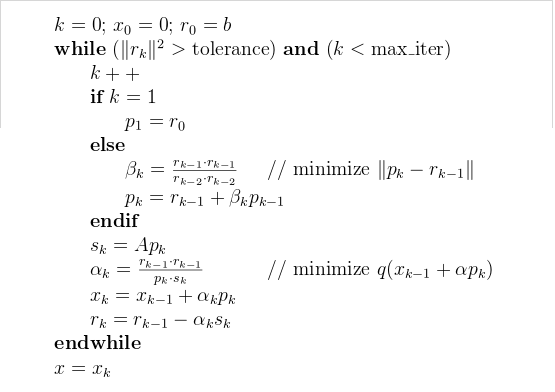
\includegraphics[width=0.75\textwidth]
		{pics/cg_par.png}
		\caption{Algoritma Conjugate Gradient Method.}
		\label{fig:cg}
	\end{figure}
	
	Program yang digunakan pada eksperimen ini merupakan program bawaan dari CUDA (NVIDIA).  Sejak CUDA versi 7.0 NVIDIA menyertakan contoh program Conjugate Gradient yang menggunakan \textit{library} CUBLAS dan CUSPARSE.  Program dimodifikasi agar dapat menerima masukan berupa ukuran array yang digunakan dan menampilkan waktu yang diperlukan dalam 1 iterasi.
%-----------------------------------------------------------------------------%
\section{Eksperimen}
%-----------------------------------------------------------------------------%

Pada eksperimen 1, kode sumber hanya dimodifikasi agar dapat menerima argumen berupa ukuran array.  Pada eksperimen 2 kode sumber dimodifikasi agar ukuran array mempengaruhi nilai A dan b.  Berikut adalah potongan kode yang dimodifikasi.

\begin{figure}
	\centering
	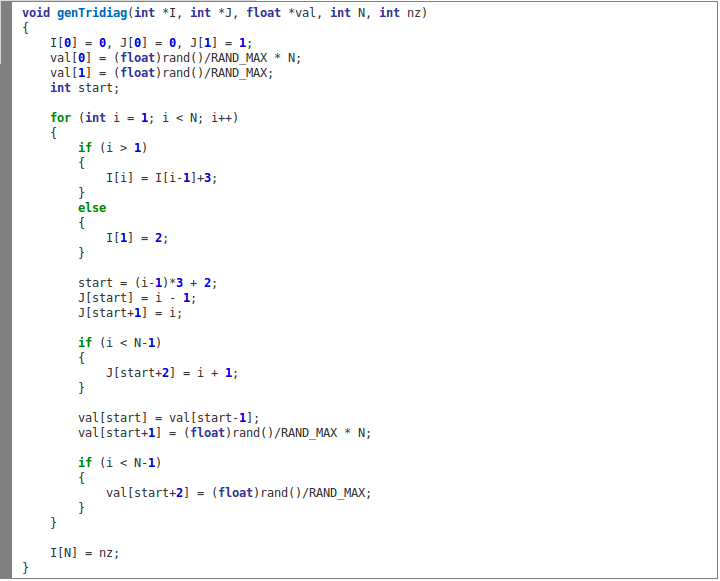
\includegraphics[width=1\textwidth]
	{pics/code1}
	\caption{Modifikasi nilai A}
	\label{fig:code1}
\end{figure}

\begin{figure}
	\centering
	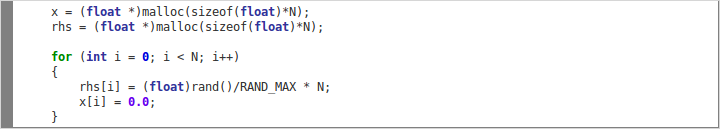
\includegraphics[width=1\textwidth]
	{pics/code2}
	\caption{Modifikasi nilai b}
	\label{fig:code2}
\end{figure}

Eksperimen dilakukan dengan menggunakan variasi ukuran array 512, 1024, 2048, dan 4096.  Gambar dibawah adalah contoh keluaran program.

\begin{figure}
	\centering
	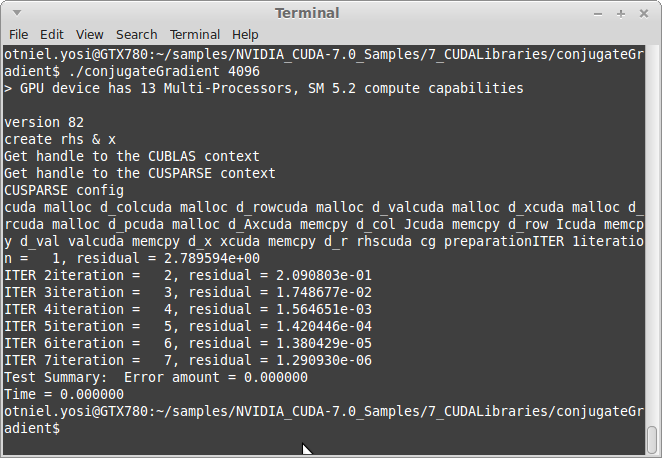
\includegraphics[width=1\textwidth]
	{pics/cudacg_4096}
	\caption{Eksperimen 1 dengan ukuran array 4096}
	\label{fig:cgcuda1}
\end{figure}

\begin{figure}
	\centering
	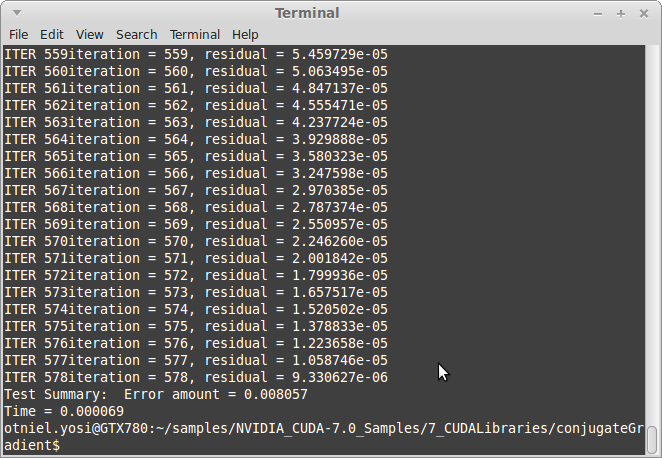
\includegraphics[width=1\textwidth]
	{pics/cudacg_4096_2}
	\caption{Eksperimen 2 dengan ukuran array 4096}
	\label{fig:cgcuda2}
\end{figure}

Gambar di bawah menampilkan grafik hasil eksperimen 1 dan 2.  Terlihat bahwa nilai pada array mempengaruhi unjuk kerja.  Namun demikian hasil keseluruhan menunjukkan bahwa implementasi Conjugate Gradient yang digunakan sangatlah efisien.

\begin{figure}
	\centering
	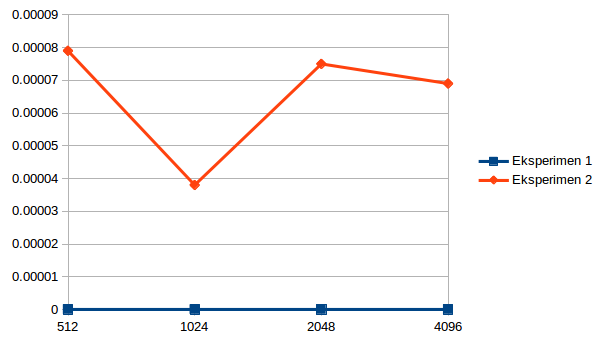
\includegraphics[width=1\textwidth]
	{pics/cg_graph}
	\caption{Unjuk kerja Conjugate Gradient dengan CUDA}
	\label{fig:cggraph}
\end{figure}

Hasil eksperimen di atas jauh mengungguli unjuk kerja Conjugate Gradient dengan MPI.  Hal ini menurut kami juga dipengaruhi oleh \textit{library} CUBLAS dan CUSPARSE yang digunakan pada implementasi Conjugate Gradient dengan CUDA karena \textit{library} tersebut merupakan \textit{library} yang cukup matang untuk operasi matriks dan vektor.

\begin{figure}
	\centering
	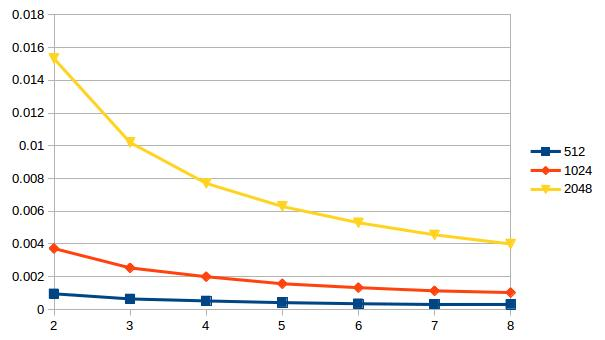
\includegraphics[width=1\textwidth]
	{pics/cg_nbcr}
	\caption{Unjuk kerja Conjugate Gradient dengan MPI pada cluster NBCR dengan variasi jumlah processor dan ukuran array}
	\label{fig:cgmpi}
\end{figure}

%-----------------------------------------------------------------------------%
\section{Kesimpulan}
%-----------------------------------------------------------------------------%

\begin{itemize}
	\item GPU (CUDA) jauh lebih efisien dibanding cluster CPU (MPI) untuk menjalankan algoritma Conjugate Gradient Method.
	\item \textit{Library} CUBLAS dan CUSPARSE sangat efektif untuk digunakan pada program yang membutuhkan operasi matriks dan vektor.
\end{itemize}